\subsection*{Worse Case of Two Samples}
If the first grouping test is positive, the samples had to be retested individually. From the method above, we considered a special case of testing: If all of the samples tested before the last one got a negative result, we assume that the last sample must be positive. But in reality, the samples may not be tested one by one but simultaneously. Which means that this special case may not exist in reality, for example, in a sample of 2, for 1 of the samples positive, 1 of the samples negative.  The probability is $p(1 -− p)$. The case for only 2 test is required as the last sample must be positive will not be considered, such that there will only be neither 1 test or 3 tests used in every group.
\\
\\
Similar to the ideal 2 sample test, we consider the following possibilities:

\begin{itemize}
  \item For all the samples negative. The probability is $(1-p)^2$. Only 1 test is required.
  \item For 1 of the samples positive, 1 of the samples negative. The probability is $p(1-p)$. 3 tests is required. 
  \item For all the samples positive. The probability is $p^2$. 2 tests is required.
\end{itemize}
The new expected number of test will be given out by:
\\
\begin{displaymath}
T(p)=3p^2 + 3p(1-p) \times 2 + 1(1-p)^2
\end{displaymath}
\\
Simplifying $T(p)$, we get:
\\
\begin{displaymath}
T(p)=-2p^2+4p+1
\end{displaymath}
\\
For solving $T(p)=2$, we get:
\\
\begin{center}
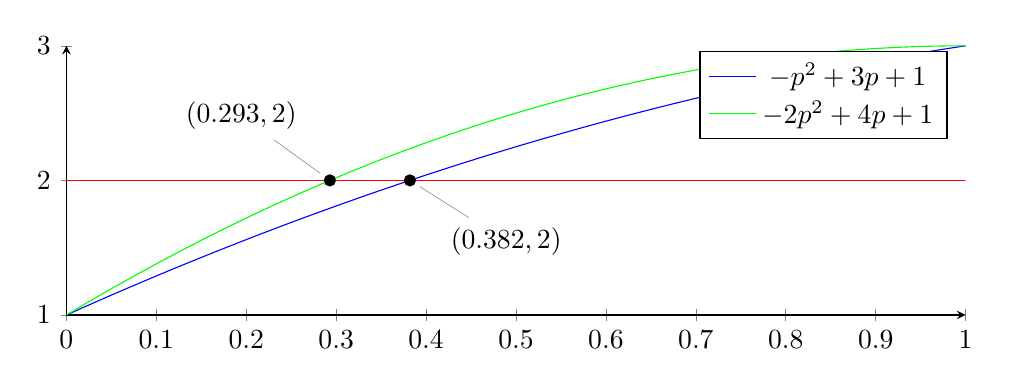
\begin{tikzpicture}
\begin{axis}[
    axis lines = left,
    ytick={0,1,2,3},
    xtick={0,0.1,0.2,0.3,0.4,0.5,0.6,0.7,0.8,0.9,1},
    height=5cm,
    width=13cm,
]

%Here the blue parabola is defined
\addplot [
    domain=-0:1, 
    samples=100, 
    color=blue,
    ]
    {-x^2 + 3*x + 1};
\addlegendentry{\(-p^2+3p+1\)}

%Here the red parabola is defined
\addplot [
    domain=0:1, 
    samples=100, 
    color=green,
    ]
    {-2*x^2 + 4*x + 1};
\addlegendentry{\(-2p^2+4p+1\)}

%Here y=2 is defined
\addplot [
    domain=0:1, 
    samples=100, 
    color=red,
    ]
    {2};

%Two dots are defined
\addplot[mark=*] coordinates {(0.293,2)} node[pin=120:{$(0.293,2)$}]{} ;
\addplot[mark=*] coordinates {(0.382,2)} node[pin=310:{$(0.382,2)$}]{} ;

\end{axis}
\end{tikzpicture}
\end{center}
\\
From the graph, we find that in the worse case, when the group size is equal to 2, pooling should be used only when $p<0.293$ such that the expected amount of tests used is lower than the traditional way.
\\
\\
We can compare the two expected functions by considering the difference:
\\
\begin{displaymath}
D(p)=T(p)-t(p)=-2p^2+4p+1-(-p^2+3p+1)
\end{displaymath}
\\
Solving $D(p):$
\\
\begin{displaymath}
D(p)=-p^2+p
\end{displaymath}
\\
The difference of the two equations is a cubic equation.
\\
\\
Graphing the equation:
\\
\begin{center}
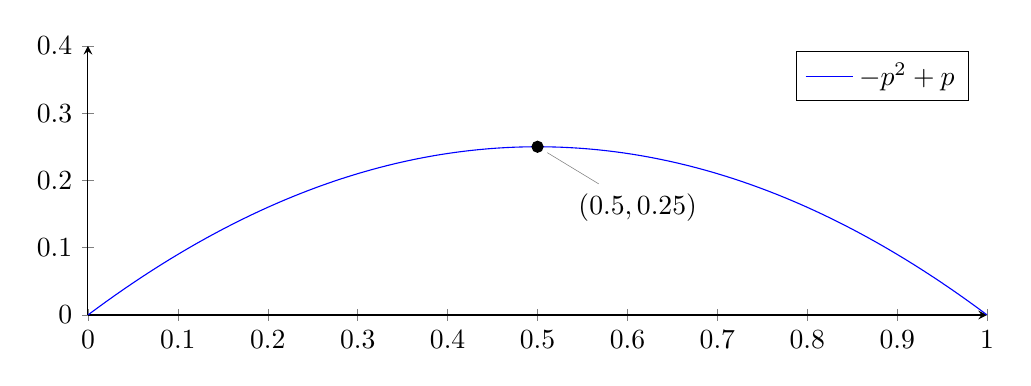
\begin{tikzpicture}
\begin{axis}[
    axis lines = left,
    ytick={0,0.1,0.2,0.3,0.4},
    ymin=0.0,ymax=0.4,
    xtick={0,0.1,0.2,0.3,0.4,0.5,0.6,0.7,0.8,0.9,1},
    height=5cm,
    width=13cm,
]

%Here the blue parabola is defined
\addplot [
    domain=0:1, 
    samples=100, 
    color=blue,
    ]
    {-x^2 +x};
\addlegendentry{\(-p^2+p\)}

%Two dots are defined
\addplot[mark=*] coordinates {(0.5,0.25)} node[pin=310:{$(0.5,0.25)$}]{} ;

\end{axis}
\end{tikzpicture}
\end{center}
\\
From the graph, we noticed that the vertex of the equation is $(0.5,0.25)$, which means that the biggest difference occurs when $p=0.5$ and the expected value of the two models differ by 0.25 tests.